\documentclass[addpoints,format=DS]{commun}

\jour{4\up{e}}
\totpoints{100}
\duree{2h00}
\presentationpoints{10}



\begin{document}

    \begin{questions}

        \question[17]\par
        \begin{minipage}{.3\linewidth}
            \begin{center}
                \begin{tikzpicture}[scale=0.4]
                    \coordinate[label=below:A](A)at(0,0);
                    \coordinate[label=below right:B](B)at(2,1);
                    \coordinate[label=right:C](C)at(2,5);
                    \coordinate[label=right:D](D)at(2,6);
                    \coordinate[label=below left:E](E)at(0,4);
                    \coordinate[label=below:H](H)at(-6,2);
                    \coordinate[label=below:I](I)at(-4,3);
                    \coordinate[label=left:F](F)at(-6,6);
                    \coordinate[label=above left:G](G)at(-4,8);
                    \coordinate(J)at(6,3);
                    \coordinate(N)at(-4,7);
                    \coordinate(M)at(-2,11);
                    \coordinate(L)at(4,9);
                    \coordinate(K)at(6,8);
                    \def\housepalette{Rainbow1}\def\housecolor{bleu}
                    \draw[fill=\housepalette-\housecolor]%
                    (B)--(I)--(G)--(D)--cycle;
                    \draw[fill=\housepalette-\housecolor]%
                    (B)--(J)--(K)--(L)--(D)--cycle;
                    \draw[fill=\housepalette-\housecolor]%
                    (D)--(L)--(M)--(G)--cycle;
                    \foreach \a in {0.1,0.2,...,0.9}{%
                        \path(G)--(D)coordinate[pos=\a](u);
                        \path(F)--(E)coordinate[pos=\a](v);
                        \draw(u)--(v);
                    }
                    \coordinate[label=below left:E](E)at(0,4);
                    \coordinate[label=right:C](C)at(2,5);
                    \coordinate[label=right:D](D)at(2,6);
                    \draw(H)--(F)--(G)--(N)--(F)--(E);
                    \draw(A)--(E)--(D)--(C)--(E);
                    
                    \tikzset{
                        seagull/.pic={
                            \draw (-6mm,0) to [bend left] (0,0) to [bend left] (6mm,0);
                        }
                    }
                    \pic[rotate=5] at (6,11) {seagull};
                    \pic[rotate=-10] at (7,12) {seagull};
                \end{tikzpicture}
            \end{center}
        \end{minipage}\hspace{0.03\linewidth}
        \begin{minipage}{.3\linewidth}
            \begin{center}
                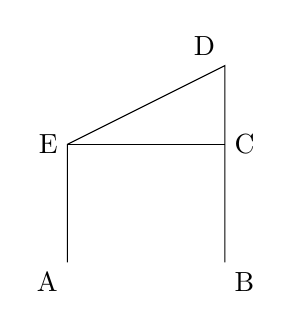
\begin{tikzpicture}[scale=0.5]
                    \coordinate[label=below left:A](A)at(0,0);
                    \coordinate[label=left:E](E)at(0,3);
                    \coordinate[label=right:C](C)at(4,3);
                    \coordinate[label=below right:B](B)at(4,0);
                    \coordinate[label=above left:D](D)at(4,5);
                    \tkzMarkRightAngle(A,E,C)
                    \tkzMarkRightAngle(E,C,B)
                    \draw(A)--(E)--(D)--(B);
                    \draw(E)--(C);
                \end{tikzpicture}
            \end{center}
        \end{minipage}\hspace{0.03\linewidth}
        \begin{minipage}{.3\linewidth}
            \begin{center}
                \textsf{EC} = 2,85 m\par
                \textsf{BC} = 2,10 m\par
                \textsf{BD} = 3,10 m\par
                \textsf{EF} = 6,10 m\par
                Le toit de la véranda est représenté par le rectangle \textsf{EDGF}.
            \end{center}
        \end{minipage}
        \begin{center}\vspace{5pt}
            \pdf[scale=0.5]{4eme_Devoir_commun_tableau1}
        \end{center}\vspace{20pt}
        \textit{On rappelle que l'aire d'un rectangle est définie par :
        aire = longueur $\times$ largeur}.
        \begin{parts}
            \part Une tâche cache le prix au m$^2$ des \og tuiles régence \fg.
            Calculer ce prix.
            \part Mélanie décide finalement de couvrir le toit de sa vérenda
            avec des tuiles romanes.\par
            Ces tuiles sont vendues à l'unité.
            \begin{subparts}
                \subpart Calculer $\textsf{DC}$.
                \subpart Calculer $\textsf{ED}$.
                \subpart Calculer la surface du toit de la vérenda.
                \subpart En déduire le nombre de tuiles que Mélanie doit acheter.
            \end{subparts}
        \end{parts}

        \vfill
        \question[9]
        \begin{minipage}[c]{.45\linewidth}
            On suppose que le mât est perpendiculaire à la coque du bateau.\par
            Calculer une valeur approchée de la hauteur du mât
            du bateau schématisé ci-contre.
        \end{minipage}\hspace{0.05\linewidth}
        \begin{minipage}[c]{.45\linewidth}
            \pdf[scale=1.8]{4eme-pythagore-calcul_mat_bateau}
        \end{minipage}

        \question[10]
        \phantom{a}
        \begin{center}
            \begin{tikzpicture}[rotate=-3, scale=1.3]
                \def\radius{1}
                \def\height{0.866}
                \def\heighttwo{\radius*2+1}
                \def\hex#1#2{%
                    \foreach\angle/\X/\xlabel in{%
                        0/A/above right,%
                        60/B/above left,%
                        120/C/left,%
                        180/D/below left,%
                        240/E/below right,%
                        300/F/right%
                    }{%
                        \ifnum#2=1
                        \path(center#1)--+(\angle:\radius)%
                        coordinate[label=\xlabel:\X](\X#1);
                        \else
                        \path(center#1)--+(\angle:\radius)coordinate(\X#1);
                        \fi
                    }
                    \draw(A#1)--(B#1)--(C#1)--(D#1)--(E#1)--(F#1)--cycle;
                }
                \coordinate(center0)at(0,0);
                \hex01
                \foreach\idangle in{1,...,6}{%
                    \coordinate(center\idangle)at(\idangle*60-30:\height*2);
                    \hex\idangle0
                }
                \coordinate(center7)at(0:\heighttwo);
                \hex70
                \coordinate(center8)at(-60:\heighttwo);
                \hex80
                \coordinate(center9)at(-30:\height*4);
                \hex90
                \foreach\centerId/\centerLabel in{%
                    0/5,%
                    1/2,%
                    2/1,%
                    3/4,%
                    4/8,%
                    5/9,%
                    6/6,%
                    7/3,%
                    8/10,%
                    9/7%
                }{%
                    \draw node at(center\centerId){\centerLabel};
                    }
                \tkzMarkAngle[size=0.3,mark=none](E0,F0,E6)
                \tkzLabelAngle[pos=0.5](E0,F0,E6){\footnotesize 120$\^\circ$}
            \end{tikzpicture}
        \end{center}
        \begin{parts}
            \part Quelle est l'image de l'hexagone 3 par la translation qui
            transforme \textsf{D} et \textsf{B} ?
            \part Quelle est l'image de l'hexagone 8 par la rotation de centre
            \textsf{F}, d'angle {120$\^\circ$} et dans le sens anti-horaire ?
        \end{parts}
    \vspace{10pt}
    \newpage

    \question[20]
    \begin{center}
        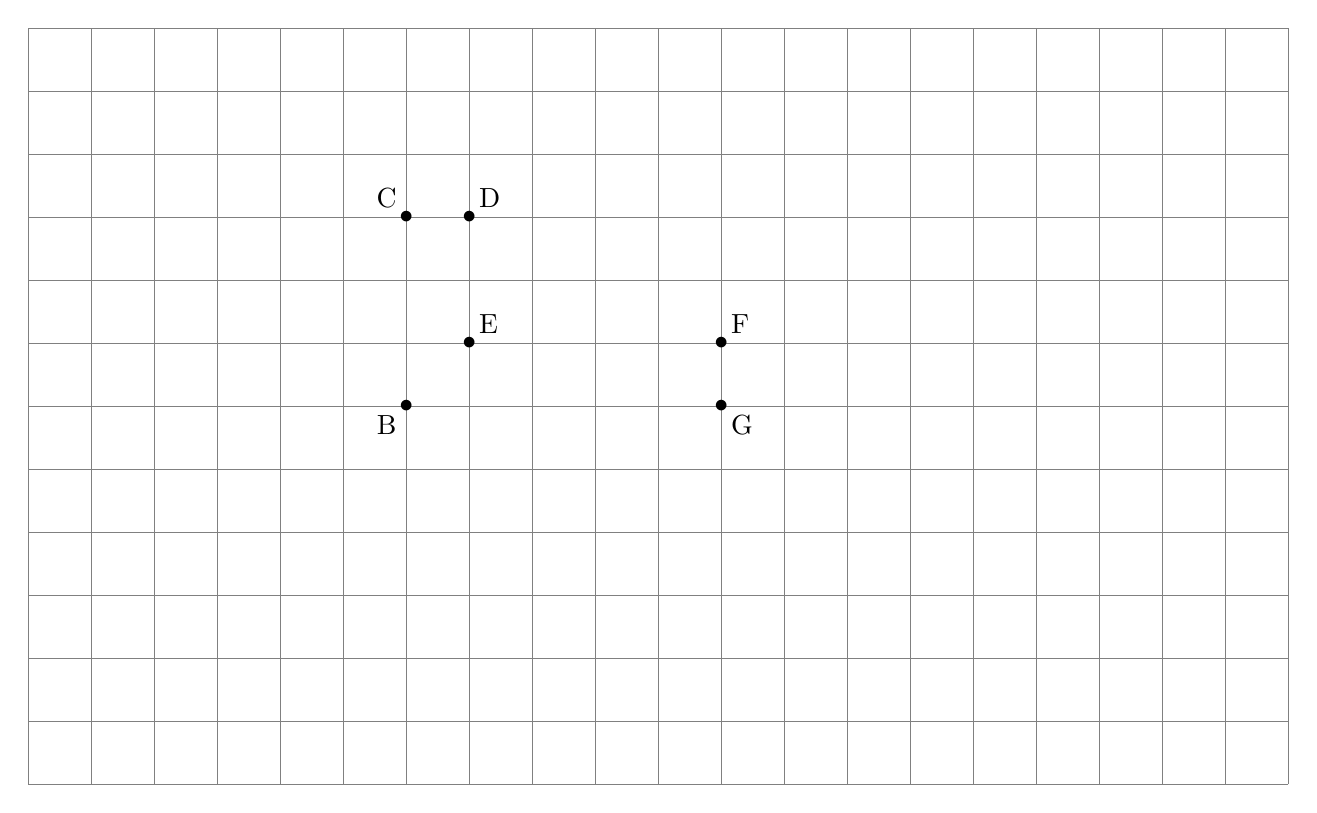
\begin{tikzpicture}[scale=0.8]
            \draw[line width=0.5 pt, gray](0,0)grid(20,12);
            \coordinate[label=below left:B](B)at(6,6);
            \coordinate[label=above left:C](C)at(6,9);
            \coordinate[label=above right:D](D)at(7,9);
            \coordinate[label=above right:E](E)at(7,7);
            \coordinate[label=above right:F](F)at(11,7);
            \coordinate[label=below right:G](G)at(11,6);
            \foreach\X in{B,C,D,E,F,G}{%
                \draw node at(\X){$\bullet$};
            }
            \tkzDrawPolygon[line width=1.2pt](B,C,D,E,F,G)
        \end{tikzpicture}
    \end{center}\par
    Tracer sur le quadrillage ci-dessus l'image du polygone
    \textsf{BCDEFG} par la translation qui transforme \textsf{G}
    et \textsf{C}.
    \vspace{20pt}

    \question[24]
    Les questions \textbf{1)} et \textbf{2)} sont indépendantes.
    \begin{parts}
        \part Effectuer les calculs suivants en donnant le résultat sous la
        forme d'une fraction irréductible.
        \begin{enumerate}[label={\Alph* =}]
            \begin{multicols}{2}
                \item$\dfrac{3}{5}+\dfrac{6}{5}\times\dfrac{7}{18}$\vspace{20pt}
                \columnbreak
                \item$8\div\dfrac{12}{5}$
            \end{multicols}
        \end{enumerate}
        \part Dans la bibliothèque de Carla, un tiers des livres sont des
        bandes dessinée, un dixième sont des manuels scolaires. Les livres
        restants sont des romans. Quelle est la proportion de roman ?
    \end{parts}

    \vfill
    \question[10]
        Une recette de cuisine indique les proportions suivantes:
        \begin{center}
            \og Deux kilogrammes de sucre pour trois kilogrammes d'abricots.\fg
        \end{center}
        \begin{parts}
            \part De quelle masse de sucre a-t-on besoin pour 7,5 kg d'abricots ?
            \part De quelle masse d'abricots a-t-on besoin pour 3 kg de sucre ?
        \end{parts}\vspace{10pt}
    \end{questions}
\end{document}